Numerical analysis courses are ubiquitous in the mechanical engineering degrees programme's firsts years in the Argentine Republic.
There are usually preceded by a course on programming fundamentals, allowing to focus the efforts of the teaching staff of the former to rely on what was taught in the later.
Unfortunately it is not unusual that in later courses the problems presented to students are limited to those 
having analytical solutions of the models, so the knowledge and practice obtained not only on the subject of numerical analysis, but also of programming as a tool, are seldom exploited at full at later courses.
In an effort to revert this trend, our course on analytical mechanics precedes those later ones and is placed immediately after those where these abilities were acquired. 
As shown by the roadmap presented in Figure \ref{fig:correlativas} for the degree on mechanical engineering at La Matanza University (UNLaM).
One reason to do so, is to put mechanical engineering students to work on the subject matter of mechanical devices quickly, capitalising what they learnt in subjects devoted to algebra, mathematical analysis, numerical calculus, and Newtonian mechanics.
Another reason is to assure the teaching staff of the subjects on the mechanics of stability, devices or fluids, that the students they receive are experienced on the tools of analytical mechanics but also on computer-based numerical analysis.
In this way the course acts as a link between the first specific mechanical courses and the basic ones.

\begin{figure}[ht]
\centering
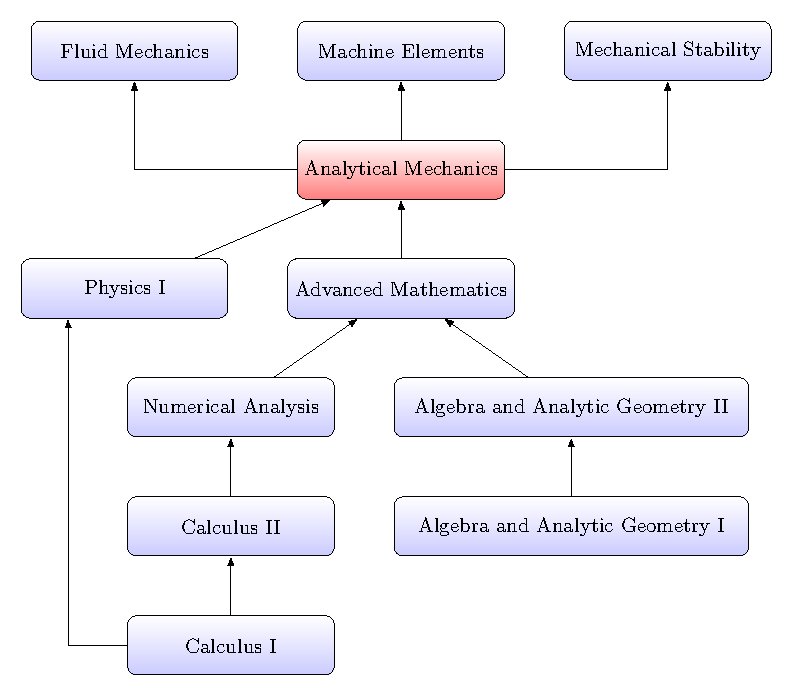
\includegraphics[width=0.9\linewidth]{figuras/ubicacion}
\caption{Preceded by subjects of algebra, calculus, and physics, analytical mechanics is the first in which such knowledge is applied to mechanical engineering.
It also serves as a foundation for subsequent specialised mechanical engineering courses.}
\label{fig:correlativas}
\end{figure}

But, why is the physics subject of analytical mechanics, also known as classical mechanics, a worthwhile tool for mechanical engineers? 
The mere statement that it confers the power to model the physics of simple mechanical systems does make it sound like a redux of Newtonian mechanics.
And it is in putting in contraposition with that another philosophy of how to understand physical mechanics that the value of the analytical approach stands appart.
Instead of an artisanal analysis of vector forces, the analytical approach is absolutely systematic.
Creativity is only required to produce a physical model out of the observation of the actual system, then it follows the same identical steps, independently of the system under study, to produce results, making it highly automatable for machines or people alike \cite{cornelius_lanczos_variational_1952}.
The creation of a physical model from observations involves simplifications, the student must determine what is important and what is not to capture the main features of the physical system.

Training this ability of students is the most demanding challenge  to the teaching staff of this course.
Once a physical model is constructed the analytical mechanics steps based on the Euler-Lagrange formalism, reviewed later in this work, produce a set of differential equations.
These can describe the dynamics or the mechanical efforts the actual system is subjected to, and next one needs only to solve them.
